For a tree $T$ and $u \in V(T)$, let 
\[
  \psi_T(u) = \max_{v \in V(T) - u} |(T, u)_{v \downarrow}| ,
\]
so $\psi_T(u)$ is the size of the largest subtree of $T$ hanging off
of the vertex $u$. We omit the subscript $T$ when the tree is
understood.

Consider the strategy for picking central nodes from an unlabelled
copy of $T \sim \UA(n, S)$ which works by simply picking the $K$ nodes
minimizing the values of $\psi$. We will write
$H^*_{\psi; K}(T^\circ)$ for such a set of nodes. This strategy was
first successfully introduced in \cite{finding-adam}, where $\psi$ is
seen as a measure of node centrality, and in which it is shown that
the root of $\UA(n)$ (which is the node labelled $u_1$) is likely to
have low $\psi$ value. In fact, it is shown that this is also true for
the root in preferential attachment trees. This centrality measure is
further studied for root-finding in different settings
\cite{ling-centrality,jog-persistence,khim-confidence}.

Specifically, the result of \cite[Theorem 3]{finding-adam} has that
for $K \ge (2.5/\eps) \log(1/\eps)$,
\[
  \Pr_{T \sim \UA(n)}\Big\{u_1 \in H^*_{\psi; K}(T^\circ)\Big\} \ge 1 - \frac{4 \eps}{1 - \eps} ,
\]
and so, for $\eps \le 1/2$, $K(\eps) \le (80/\eps) \log(1/\eps)$. The
following result indicates that $H^*_{\psi; K}$ also serves as a
root-finding algorithm for seeded uniform attachment seeds, and offers
an upper bound on the size of such vertex confidence sets.

Our proof relies on a few supporting lemmas and a classical result in
the study of P\'{o}lya urns, whose proofs and statements are given in
\appref{app}.
\begin{prop}\proplabel{heart-upper}
  There are universal constants $c, \eps_0 > 0$ for which, if
  $\eps \le \eps_0$ and
  \[
    K \ge c (1/\eps)^{2/k} \log(1/\eps) ,
  \]
  then
  \[
    \Pr\{|V(S) \cap H^*_{\psi; K}(T^\circ)| \ge 1 \} \ge 1 - \eps .
  \]
\end{prop}
\thmref{heart-upper} follows immediately.
\begin{proof}[Proof of \propref{heart-upper}]
  \begin{figure}
    \centering
    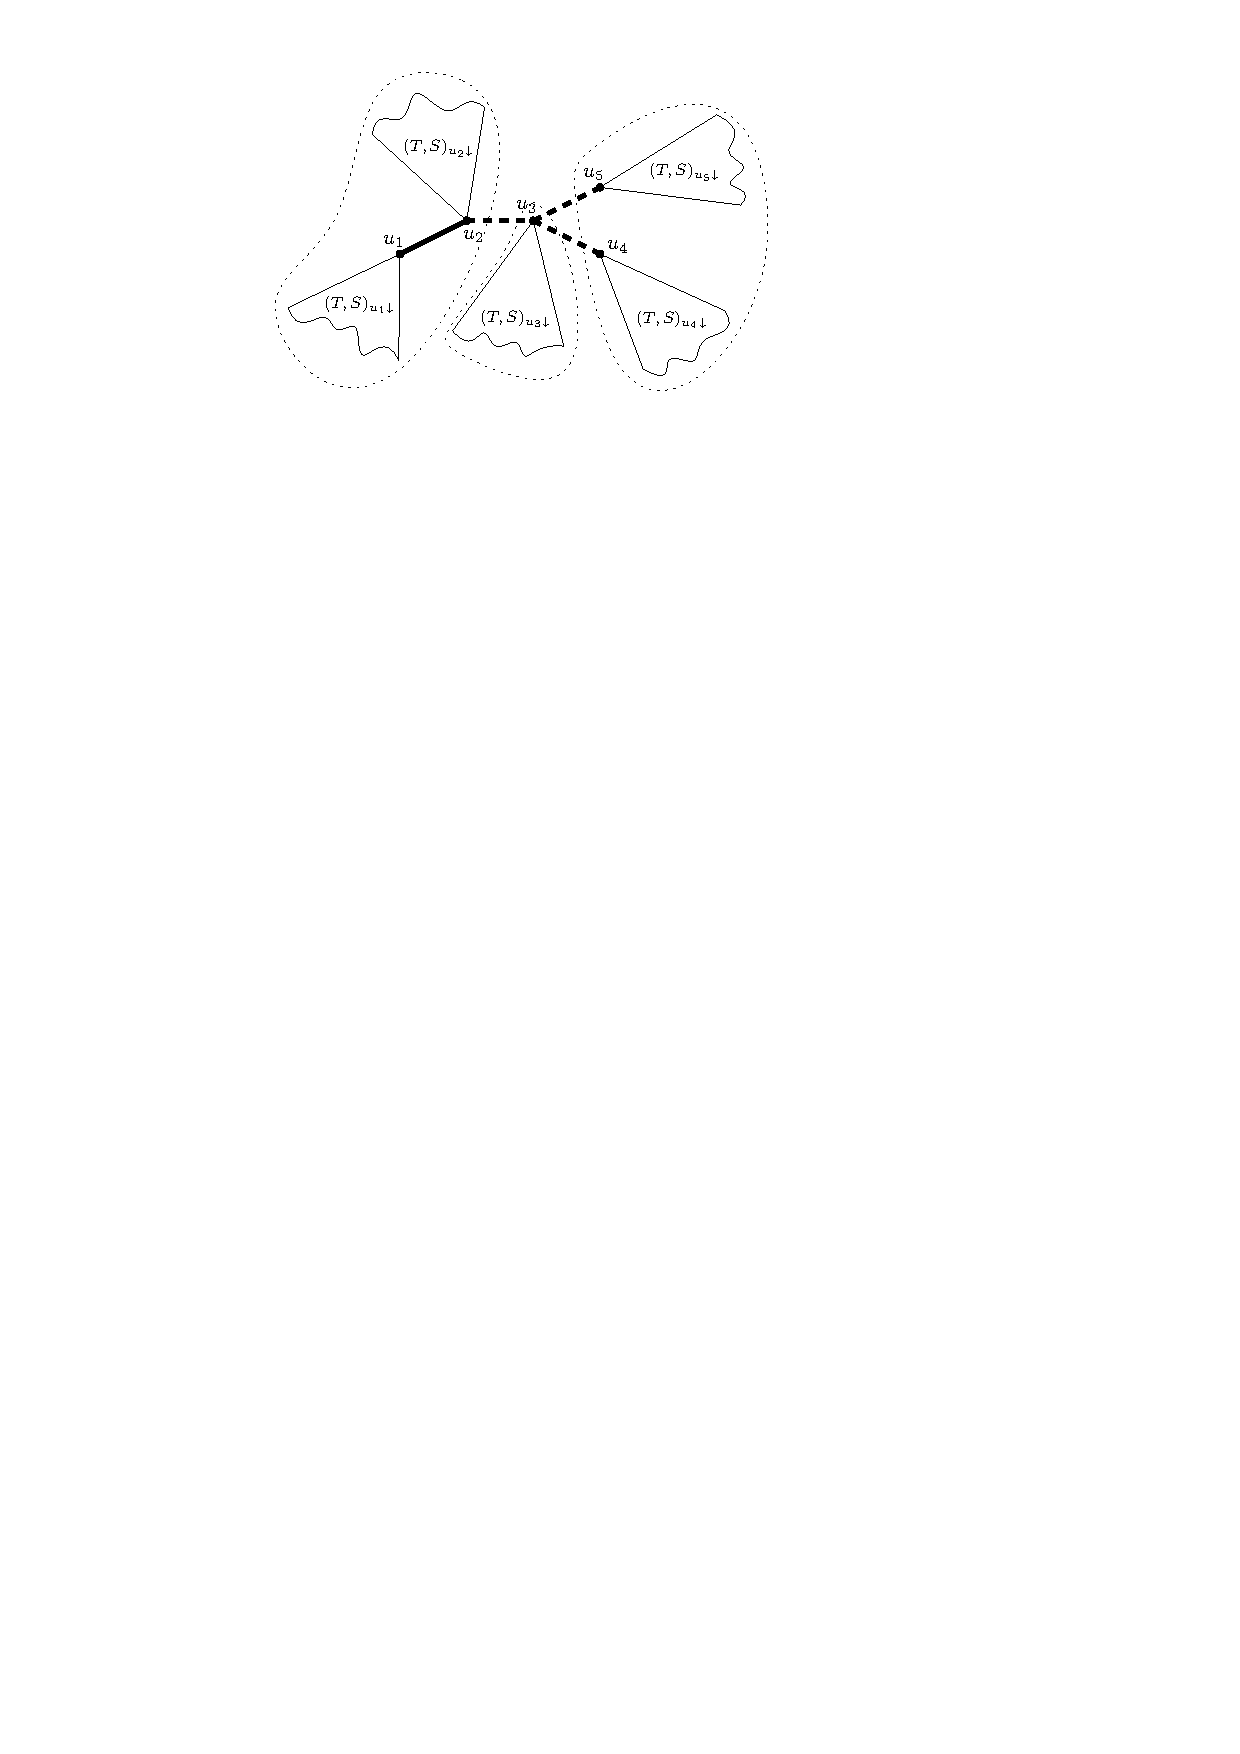
\includegraphics[width=0.6\textwidth]{centroid.pdf}
    \caption{The seed $S$ has vertex set $\{u_1, \dots, u_5\}$. The
      node $r = u_3$ is its unique centroid. The dashed edges form the
      set $\partial_S(r)$. The dotted lines outline the components of
      $S - \partial_S(r)$.}
    \figlabel{centroid}
  \end{figure}
  Let $\psi_* = \min\{\psi(u_1), \dots, \psi(u_k)\}$. If for all
  $i > K$, $\psi(u_i) > \psi_*$, then $V(S)$ intersects
  $H^*_{\psi; K}(T^\circ)$, so
  \begin{align}
    \Pr\{V(S) \cap H^*_{\psi; K}(T^\circ) = \emptyset\} &\le \Pr\{\exists i > K \colon \psi(u_i) \le \psi_*\} \notag \\
                                                        &\le \Pr\{\psi_* \ge nt\} + \Pr\{\exists i > K \colon \psi(u_i) \le nt\} , \eqlabel{phi-tail}
  \end{align}
  where $t > 0$ is to be specified later. It is a classical result
  that the seed $S$ has a centroid, \ie a node $r$ whose removal
  splits the seed into components each of size at most
  $k/2$~\cite{jordan-centroid}. Note that
  \[
    \psi_* \le \psi(r) \le \max_{C \in \sC(S - \partial_S(r))} \sum_{u \in
      C} |(T, S)_{u \downarrow}| ,
  \]
  where $\sC(G)$ denotes the set of components of a graph $G$, and
  $\partial_S(r)$ denotes all of the edges of $S$ incident to
  $r$. Now, for any $C \in \sC(S - \partial_S(r))$, we have by
  \lemref{dir-convergence} that
  \[
    \frac{1}{n} \sum_{u \in C} |(T, S)_{u \downarrow}| \overset{d}{\to} \Beta(|C|, k - |C|) ,
  \]
  as $n \to \infty$, so stochastically,
  \[
    \frac{\psi_*}{n} \le \max_{C \in \sC(S - \partial_S(r))} \Beta(|C|, k - |C|)
  \]
  and since $|C| \le k/2$ uniformly because $r$ is a centroid, then
  each such beta random variable is stochastically smaller than a
  $\Beta(k/2, k/2)$ by \lemref{beta-dom-1}. See \figref{centroid}. Let
  $f_{k/2, k/2}(x)$ be the density of a $\Beta(k/2, k/2)$ random
  variable. Using the bound
  \[
    \sqrt{\frac{2 \pi}{x}} \left(\frac{x}{e}\right)^x \le \Gamma(x) \le \sqrt{\frac{2 \pi}{x}} \left(\frac{x}{e} \right)^x e^{\frac{1}{12 x}} ,
  \]
  which holds for all $x > 0$~\cite[Equation 5.6.1]{nist}, we see that
  \[
    \mathrm{B}(k/2, k/2) = \frac{\Gamma(k/2)^2}{\Gamma(k)} \ge 2^{-k} \cdot \frac{2}{e^{1/12}} \sqrt{\frac{2 \pi}{k}} > 3^{-k} 
  \]
  for all $k \ge 1$. Then,
  \begin{align*}
    \Pr\{\psi_* \ge nt\} &\le k \Pr\{\Beta(k/2, k/2) \ge t\} \\
                                    &= k \int_{t}^1 f_{k/2, k/2}(x) \dif x \\
                              &\le k 3^k \int_0^{1 - t} (x (1 - x))^{k/2 - 1} \dif x \\
                              &\le k 3^k \int_0^{1 - t} x^{k/2 - 1} \dif x \\
                          &= 2 (1 - t)^{k/2} 3^k,
  \end{align*}
  so we can pick $t = 1 - (1/9) (\eps/4)^{2/k}$.

  To summarize, we have shown that we can bound the first term in
  \eqref{phi-tail} by
  \[
    \Pr\{\psi_*/n \ge 1 - (1/9) (\eps/4) ^{2/k}\} \le \eps/2 .
  \]
  For the second term, the argument is identical to that of
  \cite[Theorem 3]{finding-adam}. Indeed, if $T_i$ denotes the
  subgraph of $T$ containing the vertex $u_i$ after the removal of all
  edges between $\{u_1, \dots, u_K\}$, then for any $i > K$,
  \[
    \psi(u_i) \ge \min_{1 \le j \le K} \sum_{m = 1, m \neq j}^K |T_m| ,
  \]
  and by \lemref{dir-convergence},
  \[
    \frac{1}{n} \sum_{m = 1, m \neq j}^K |T_m| \overset{d}{\to} \Beta(K - 1, 1) 
  \]
  as $n \to \infty$, so that
  \begin{align*}
    \Pr\{\exists i > K \colon \psi(u_i) \le nt\} &\le K \Pr\{ \Beta(K - 1, 1) \le t\} \\
                                                                     &= K t^{K - 1} \\
                                                                     &\le K e^{- (1/9) \eps^{2/k} (K - 1)} ,
  \end{align*}
  and a little bit of arithmetic shows that we should pick
  \[
    K \ge c (1/\eps)^{2/k} \log (1/\eps)
  \]
  for universal constants $c, \eps_0 > 0$, as long as
  $\eps \le \eps_0$.
\end{proof}

Consequently, we see that
\[
  K^*(k, \ell, \eps) \le c (1/\eps)^{2/k} \log (1/\eps) .
\]

We note that $H^*_{\psi; K}(T^\circ)$ can be computed in $O(n)$ time.
